\section{Introduction}

Recent advancements in Large Language Models (LLMs) have shown impressive performance across a wide range of tasks~\citep{zhao2023survey, li2024graphreader, he2024chinesesimpleqa}. Driven by vast amounts of data and efficient training, state-of-the-art LLMs demonstrate robust capabilities in following general instructions and achieving alignment with human preferences~\citep{ouyang2022training,li20242d,huang2025musc}.
However, despite these successes, they still face significant challenges when it comes to complex instruction following~\citep{jiang2023followbench,wen2024benchmarking}, which requires simultaneous satisfaction of multiple constraints. The ability to reliably execute such complex instructions is fundamental for LLMs to be deployed in sophisticated real-world scenarios, where user intent is inherently nuanced and multi-faceted.

High quality instruction data is essential for instruction alignment. Existing datasets of complex instructions primarily originate from two sources: 1) Curated data from open-source datasets or human annotations~\citep{zhou2024lima,zhang2024cfbench}, which are resource-intensive and \textbf{lacking scalability}, and 2) Transforming simple instructions into complex ones automatically using proprietary LLMs~\citep{xu2023wizardlm,sun2024conifer}. 
While the automatic methods improve scalability, the generated constraints are often recombinations of few-shot examples, resulting in \textbf{limited diversity}.
Moreover, these constraints may have \textbf{low relevance} to the target output, failing to reflect real-world scenarios, as they are derived without considering the actual response's deficiencies.

\begin{figure}[pos=t]
    \centering
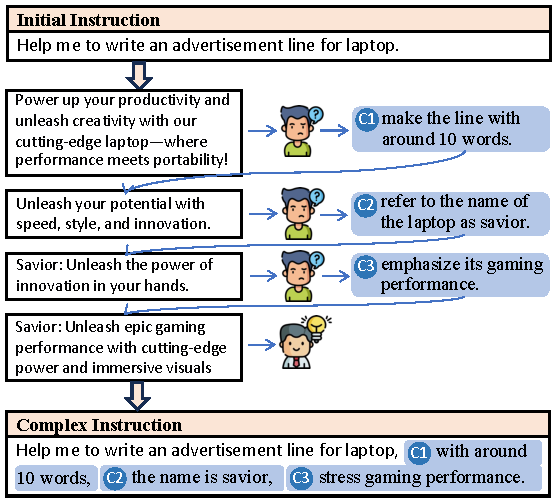
\includegraphics[width=0.86\linewidth]{source/intro.pdf}
    \caption{An illustration of humans iteratively refining instructions for higher complexity to better align with human preference.}
    \label{fig: intro}
\end{figure}

% where human iteratively refine instructions to be more complex, as shown in Figure \ref{fig: intro}.

Recently, back-translation, which involves translating text from the target response back into the source instruction, has been proposed to generate scalable and diverse instructions from human-written corpora~\citep{sennrich2015improving,hoang2018iterative,zheng2024kun,li2023self}. 
% Some studies have explored how back-translation can be leveraged to better generate instructions for fine-tuning large models~\cite{li2023self,zheng2024kun,nguyen2024better}. 
However, these methods typically focus on generating \textbf{simple instructions}, and one-way back-translation cannot fully explore the rich knowledge contained in the human corpus.

% To address the scalability and diversity of producing complex instructions,
In this paper, we propose a \textbf{Document-grounded Iterative Refinement (DIR)} framework for generating high-quality complex instructions.
Specifically, our approach is based on two key observations. First, human-written documents contain massive human preferences that can be converted into specific constraints, such as formatting conventions. Second, humans often refine complex instructions iteratively based on feedback from model outputs. As illustrated in Figure~\ref{fig: intro}, simple instructions are progressively adjusted and enriched to better align with human preferences. This iterative process plays a critical role in crafting effective complex instructions.

Therefore, our DIR framework incorporates both document-based knowledge and iterative judgment process to construct complex instructions. 
The framework consists of two key steps: 1) \textbf{Initial Instruction Generation}, where the model generates initial instructions based on the document content; 2) \textbf{Iterative Instruction Refinement}, where instructions are iteratively refined with LLM-as-judge guidance by comparing model outputs with the document, to identify and incorporate valuable constraints. This process enables us to generate more challenging instructions that align more closely with real-world scenarios. With this approach, we have curated \textbf{DIR-10K}, a high-quality complex instruction dataset.

Building upon this data, we further propose a \textbf{constraint-aware optimization pipeline} to effectively achieve instruction alignment. First, we perform Supervised Fine-Tuning (SFT) on complex instruction-response pairs curated by LLM-as-judge. Second, we employ constraint-aware Reinforcement Learning (RL) with a hybrid reward system: a model-based reward for soft constraints and a rule-based reward for hard constraints. Notably, the reward model is trained by leveraging response pairs generated during the iterative refinement process, and therefore does not require additional annotation. 

We validate our approach across various models. Experimental results demonstrate that our approach achieves significant improvements in both general and complex instruction-following tasks, thereby verifying its effectiveness. 

In summary, our contributions are as follows: 

\begin{itemize}[leftmargin=4mm]
    \item We propose the \textbf{DIR} framework, which leverages an LLM-as-judge mechanism to iteratively refine complex instructions by comparing with human-crafted documents.
    
    \item We release \textbf{DIR-10K}, a high-quality complex instruction dataset curated via our framework that achieves better alignment with real-world requirements. 
    
    \item We develop a \textbf{constraint-aware optimization pipeline} (SFT+RL) featuring a hybrid reward system that effectively aligns LLMs with complex constraints.
    
    \item Empirical results demonstrate that our fine-tuned models significantly outperform existing state-of-the-art methods across multiple instruction-following benchmarks.
\end{itemize}